\section{The Inspiration}

\frame
{
	\begin{center}
		\LARGE The Inspiration: Mimicry
	\end{center}
}

\frame
{
	\frametitle{The Inspiration: Mimicry}
	\framesubtitle{History}
	
	\begin{itemize}
		\item Henry W. Bates first published in 1862.
			\begin{itemize}
				\item \textbf{Content:} Similarity and dissimilarity between Heliconiinae and Ithomiinae butterflies. 
			\end{itemize}
		\item Bates collected 94 species of butterfly.
		\item Grouped according to similar appearance.
		\item \textbf{Discovery:} Appearance: similar, Morphological feature: different species.
		\item 67 of 94: Ithomiinae.
		\item 27 of 94: Heliconiinae.
	\end{itemize}
}

\subsection{Batesian Mimicry}

\frame
{
	\frametitle{The Inspiration: Mimicry}
	\framesubtitle{Batesian Mimicry}
	
	\begin{itemize}
		\item Heliconiids are,
			\begin{itemize}
				\item conspicuously colored
				\item extremely abundant 
				\item slow in mobility.
			\end{itemize}
		\item Predators, insectivorous birds do not prey on Heliconiids.
			\begin{itemize}
				\item \textbf{Reason:} Inediblity and unpalatability.
			\end{itemize}
		\item Heliconiids are easily recalled by predators. 
			\begin{itemize}
				\item Reason: Conspicuous coloration.
				\item Color acts as warning.
			\end{itemize}
		\item Ithomiinae and Pieridae are,
			\begin{itemize}
				\item edible 
				\item palatable
				\item pretend like Heliconiids, enjoy protection.
			\end{itemize}
	\end{itemize}
}

\frame
{
	\frametitle{The Inspiration: Mimicry}
	\framesubtitle{Batesian Mimicry}
	
	\begin{itemize}
		\item According to Wilcker:
			\begin{itemize}
				\item Actor is a mime.
				\item False representation of warning pattern: Mimicry.
				\item Bates: First to point out, so Batesian Mimicry.
			\end{itemize}
		\item \textbf{Model:} Animal avoided by predator for unpalatable behavior.
		\item \textbf{Mimic:} Imitating animal.
	\end{itemize}
}

\frame
{
	\frametitle{Batesian Mimicry}
	\framesubtitle{Plate from Bates (1862)}
	
	\begin{figure}[H]
		\centering
		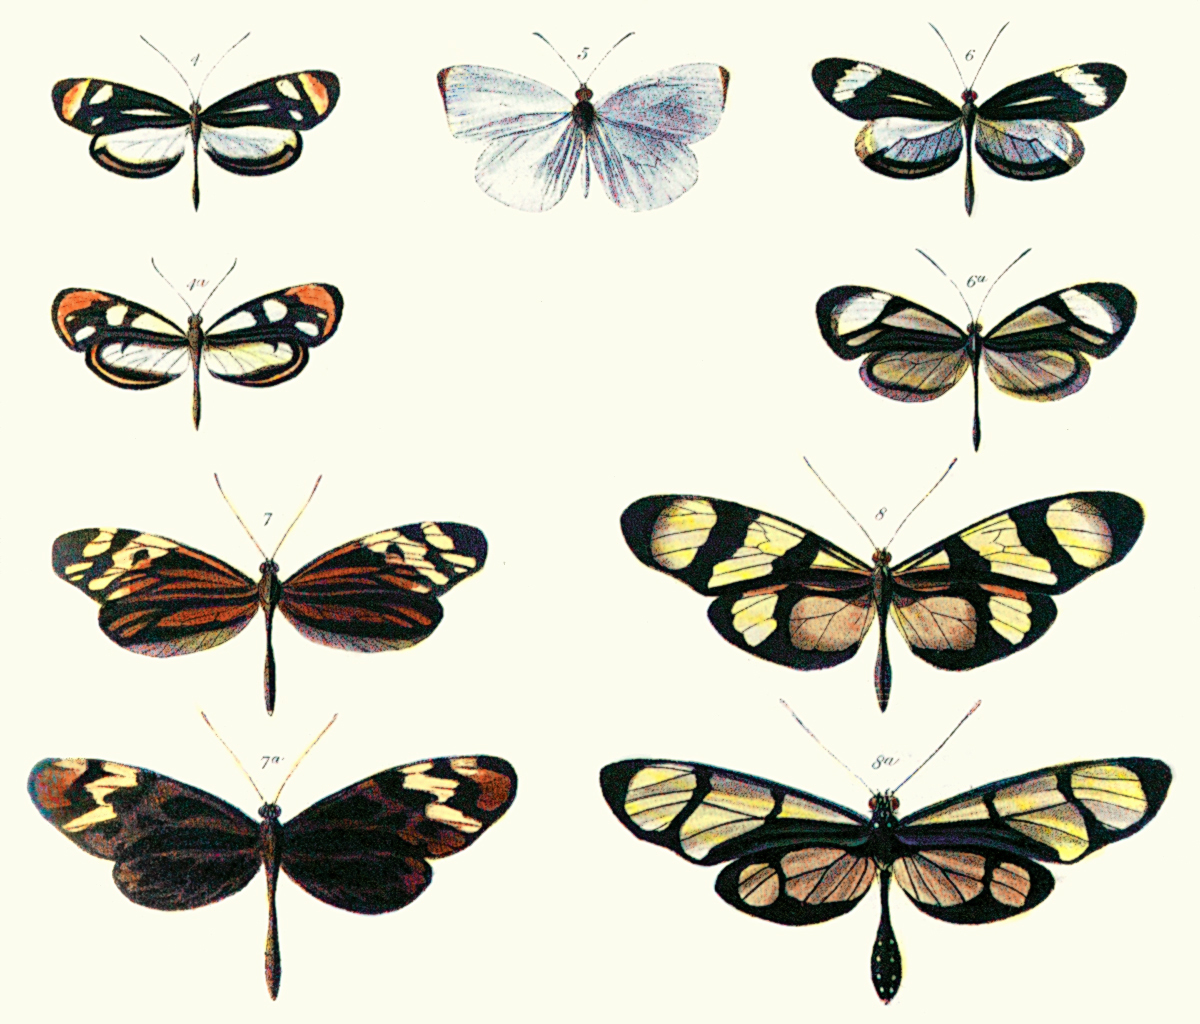
\includegraphics[scale=0.6]{../tex/images/Batesplate_ArM}
		\caption{Plate from Bates (1862) illustrating Batesian mimicry between Dismorphia species (top row, third row) and various Ithomiini (Nymphalidae) (second row, bottom row).}
		\label{fig:batesian-butterfly}
	\end{figure}
}

\subsection{Mullerian Mimicry}

\frame
{
	\frametitle{Mullerian Mimicry}
	
	\begin{itemize}
		\item Two inedible unrelated butterfly species have similar appearance. 
		\item Bates: Unable to explain.
		\item Explanation: from Fitz Muller in 1878.
		\item Muller's research was also in Brazil.
	\end{itemize}

\textbf{Explanation:}
	\begin{itemize}
		\item Predator's limited memory.
		\item Inedible species loose number.
		\item Save loss and survival of species:
			\begin{itemize}
				\item inedible, different family 
				\item evolve to have similar appearance.
			\end{itemize}
		\item Phenomenon: Mullerian mimicry, named after Fritz Muller.
	\end{itemize}
}

\frame
{
	\frametitle{Mullerian Mimicry}
	\framesubtitle{Viceroy and Monarch}

	\begin{figure}[H]
		\centering
		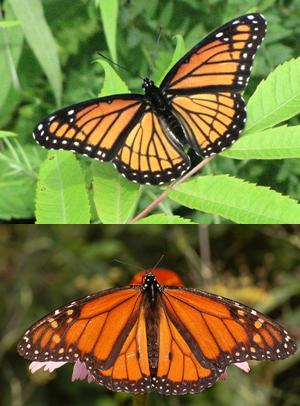
\includegraphics[scale=0.5]{../tex/images/BatesMimButter}
		\caption{A very well-known example of mimicry. Viceroy (top). Unpalatable Monarch (bottom). Image source: \href{http://en.wikipedia.org/wiki/Mullerian_mimicry}{Wikipedia}}
		\label{fig:mullerian-butterfly}
	\end{figure}

}

\subsection{Evolutionary Dynamics}

\frame
{
	\frametitle{Evolutionary Dynamics}
	\framesubtitle{Punctuated Equilibrium}

	Most sexually reproducing species remain:
	\begin{itemize}
		\item extended state of \textit{stasis}.
		\item Little evolutionary change in most geological history.
	\end{itemize}
	
	Cladogenesis:
	\begin{itemize}
		\item Process of speciation.
		\item One split into two distinct species.
		\item In geological time:
			\begin{itemize}
				\item Discontinuous change
				\item Not gradual transformation
			\end{itemize}
	\end{itemize}
}

\frame
{
	\frametitle{Evolutionary Dynamics}
	\framesubtitle{Phyletic Gradualism}

	\begin{itemize}
		\item Continued adaptation to new environmental and biological selection pressure.
		\item Gradually becoming new species.
	\end{itemize}
	
	Phyletic gradualism holds,
	\begin{itemize}
		\item Species population changes gradually.
		\item No clear demarcation between ancestral and descendant species.
		\item Gradually changing lineage is divided arbitrarily.
		\item Evolution is 
			\begin{itemize}
				\item smooth
				\item steady
				\item incremental
				\item but not necessary constant and slow rate in geological time scale.
			\end{itemize}
	\end{itemize}
}

\frame
{
	\frametitle{Evolutionary Dynamics}
	\framesubtitle{Punctuated Equilibrium vs. Phyletic Gradualism}

	\begin{figure}[H]
		\centering
		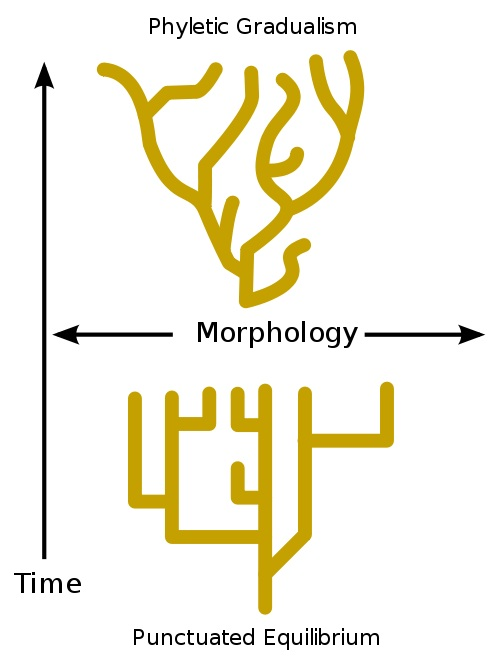
\includegraphics[scale=0.3]{../tex/images/Punctuated-equilibrium}
		\caption{Punctuated equilibrium (bottom), phyletic gradualism (top). Image source: \href{http://en.wikipedia.org/wiki/Punctuated_equilibrium}{Wikipedia}}
		\label{fig:punctuated-equilibrium}
	\end{figure}
}

\frame
{
	\frametitle{Evolutionary Dynamics}
	\framesubtitle{Turner's Two Stage Model}

	\begin{itemize}
		\item Turner: Synthetic theory.
		\item Originated from Poulton and Nicholson.
		\item Mimicry arises in two steps:
			\begin{enumerate}
				\item A comparatively large mutation achieves a good approximate resemblance.
				\item A gradual evolutionary change refines the resemblance to a higher degree of perfection.
			\end{enumerate}
		\item Theory also applied to Mullerian Mimicry.
	\end{itemize}
}

\subsubsection{Mimicry Ring}

\frame
{
	\frametitle{Mimicry Ring}
	
	\begin{itemize}
		\item Examine the local butterfly fauna in any area of the world
		\begin{itemize}
			\item all the aposomatic species
			\item limited number of different patterns
			\item normally far smaller than the number of species.
		\end{itemize}
		\item Mullerian mimicry ring: 
			\begin{itemize}
				\item Each cluster of species
				\item all sharing a common pattern
			\end{itemize}		
		\item All the rain forest in South and Central America,
		\begin{itemize}
			\item most of the long winged butterflies (ithomiids, danaids and heliconids) 
			\item belong to one of only five different rings.
		\end{itemize}
	\end{itemize}	
}